%%%%%%%%%%%%%%%%%%%%%%%%%%%%%%%%%%%%%%%%%%%%%%%%%%%%%%%%%%%%%%%%%%%%%%%%%%%%%%%%%%
\begin{frame}[fragile]\frametitle{}
\begin{center}
{\Large Background}
\end{center}
\end{frame}

%%%%%%%%%%%%%%%%%%%%%%%%%%%%%%%%%%%%%%%%%%%%%%%%%%%%%%%%%%%
\begin{frame}[fragile]\frametitle{Traditional vs. Machine Learning?}
\begin{center}
\includegraphics[width=0.8\linewidth,keepaspectratio]{tradml}
\end{center}
\end{frame}

%%%%%%%%%%%%%%%%%%%%%%%%%%%%%%%%%%%%%%%%%%%%%%%%%%%%%%%%%%%
\begin{frame}[fragile]\frametitle{Why Machine Learning?}
\begin{itemize}
\item Problems with High Dimensionality
\item Hard/Expensive to program manually
\item Job \$\$\$
\end{itemize}
%\begin{center}
%\includegraphics[width=0.45\linewidth,keepaspectratio]{hp}
%\end{center}
\end{frame}



%%%%%%%%%%%%%%%%%%%%%%%%%%%%%%%%%%%%%%%%%%%%%%%%%%%
\begin{frame}[fragile] \frametitle{ML vs DL: What's the difference?}
Deep learning algorithms attempt to learn (multiple levels of) representation by using a hierarchy of multiple layers
\begin{center}
\includegraphics[width=\linewidth,keepaspectratio]{dlfeat1}
\end{center}
\tiny{(Reference: https://www.xenonstack.com/blog/static/public/uploads/media/machine-learning-vs-deep-learning.png)}

\end{frame}

%%%%%%%%%%%%%%%%%%%%%%%%%%%%%%%%%%%%%%%%%%%%%%%%%%%%%%%%%%
\begin{frame}[fragile] \frametitle{Use Deep Learning When \ldots}

\begin{itemize}
\item You have lots of data (about 10k+ examples)
\item The problem is ``complex'' - speech, vision, natural language
\item The data is unstructured 
\item Techniques to model `ANY' function given `ENOUGH' data.
% \item You need the absolute ``best'' model
\end{itemize}
\tiny{(Ref: Introduction to TensorFlow 2.0 - Brad Miro)}
\end{frame}

%%%%%%%%%%%%%%%%%%%%%%%%%%%%%%%%%%%%%%%%%%%%%%%%%%%%%%%%%%%
\begin{frame}[fragile]\frametitle{Relationship between AI, ML, DL}
\begin{center}
\includegraphics[width=\linewidth,keepaspectratio]{ai1}
\end{center}
{\tiny (Ref: https://blogs.nvidia.com/blog/2016/07/29/whats-difference-artificial-intelligence-machine-learning-deep-learning-ai/)}
\end{frame}

% %%%%%%%%%%%%%%%%%%%%%%%%%%%%%%%%%%%%%%%%%%%%%%%%%%%%%%%%%%%
% \begin{frame}[fragile]\frametitle{Get Time Sense}
% \begin{center}
% \includegraphics[width=\linewidth,keepaspectratio]{llm117}
% \end{center}

% {\tiny (Ref: Preparing your board for Generative AI - KPMG)}
% \end{frame}

%%%%%%%%%%%%%%%%%%%%%%%%%%%%%%%%%%%%%%%%%%%%%%%%%%%%%%%%%%%
\begin{frame}[fragile]\frametitle{What is Deep NLP}
\begin{center}
\includegraphics[width=0.8\linewidth,keepaspectratio]{nlp4}

\tiny{(Ref: Deep Learning and NLP A-Z - Kirill Eremenko)}

\tiny{(Note: Size is not indicative of importance)}
\end{center}

Seq2Seq is heavily used technique of DNLP for sequence to sequence modeling, eg Translation, Q \& A, etc. Thats the basis of Large Language Models (LLMs)

	% \begin{itemize}
	% \item Green part is NLP (rule based, linguistic)
	% \item Blue part is Deep Learning not applied to NLP
	% \item Purple is Deep NLP (DNLP), NN applied for NLP use cases
	% \item Seq2Seq is heavily used technique of DNLP for sequence to sequence modeling, eg Translation, Q \& A, etc.
	% \end{itemize}
	

\end{frame}


%%%%%%%%%%%%%%%%%%%%%%%%%%%%%%%%%%%%%%%%%%%%%%%%%%%%%%%%%%%%%%%%%%%%%%%%%%%%%%%%%%
\begin{frame}[fragile]\frametitle{}
\begin{center}
{\Large Overview of Large Language Models}
\end{center}
\end{frame}



%%%%%%%%%%%%%%%%%%%%%%%%%%%%%%%%%%%%%%%%%%%%%%%%%%%%%%%%%%%
\begin{frame}[fragile]\frametitle{Typical Machine Learning Classification}
	\begin{itemize}
	% \item Questions are converted to bag of words (a vocab long vector, having frequency of specific words at their places)
		\item Each text item thus gets converted to fixed size vector, thus features.
		\item In training, weights are computed based on the given target.
		\item Once model is ready, it is able to answer target, say, Yes or No to unseen text.
			\end{itemize}
\begin{center}
\includegraphics[width=\linewidth,keepaspectratio]{nlp11}

\tiny{(Ref: Deep Learning and NLP A-Z - Kirill Eremenko)}
\end{center}

\end{frame}

%%%%%%%%%%%%%%%%%%%%%%%%%%%%%%%%%%%%%%%%%%%%%%%%%%%%%%%%%%%
\begin{frame}[fragile]\frametitle{Evolution of Vectorization}

Vectors can be statistical (frequency based) or Machine/Deep Learning (supervised) based. Simple to complex.

\begin{center}
\includegraphics[width=\linewidth,keepaspectratio]{chatgpt30}
\end{center}				
{\tiny (Ref: Analytics Vidhya https://editor.analyticsvidhya.com/uploads/59483evolution\_of\_NLP.png)}

\end{frame}


%%%%%%%%%%%%%%%%%%%%%%%%%%%%%%%%%%%%%%%%%%%%%%%%%%%%%%%%%%%
\begin{frame}[fragile]\frametitle{How to Vectorize? Representing words by their context}



\begin{center}
\includegraphics[width=0.9\linewidth,keepaspectratio]{bert6}
\end{center}		  


{\tiny (Ref: CS224n: Natural Language Processing with Deep Learning - Christopher Manning)}

\end{frame}




%%%%%%%%%%%%%%%%%%%%%%%%%%%%%%%%%%%%%%%%%%%%%%%%%%%%%%%%%%%
\begin{frame}[fragile]\frametitle{Word vectors}

\begin{columns}
    \begin{column}[T]{0.5\linewidth}
			\begin{itemize}
			\item Dense vector for each word
			\item Called distributed representation, word embeddings or  word representations 
			\item Test: similar to vectors of words that appear in similar contexts
			\end{itemize}
    \end{column}
    \begin{column}[T]{0.5\linewidth}
			\begin{center}
			\includegraphics[width=0.4\linewidth,keepaspectratio]{bert7}
			\end{center}		  
    \end{column}
  \end{columns}
% {\tiny (Ref: CS224n: Natural Language Processing with Deep Learning - Christopher Manning)}

\end{frame}
% %%%%%%%%%%%%%%%%%%%%%%%%%%%%%%%%%%%%%%%%%%%%%%%%%%%%%%%%%%%
% \begin{frame}[fragile]\frametitle{Seq2Seq architecture}

% \begin{center}
% \includegraphics[width=\linewidth,keepaspectratio]{nlp13}

% \tiny{(Ref: Deep Learning and NLP A-Z - Kirill Eremenko)}
% \end{center}

% For Seq2seq last 2 options are possible. We are going ahead with the 2nd last. Last one has fixed input and same size output.

% \end{frame}

%%%%%%%%%%%%%%%%%%%%%%%%%%%%%%%%%%%%%%%%%%%%%%%%%%%%%%%%%%%
\begin{frame}[fragile]\frametitle{Seq2Seq architecture}

\begin{center}
\includegraphics[width=0.8\linewidth,keepaspectratio]{nlp14}

\tiny{(Ref: Deep Learning and NLP A-Z - Kirill Eremenko)}
\end{center}
During training, Encoder is fed with Questions and decoder with Answers. Weights in gates, hidden states get settled. During testing for each sequence of input, encoder results in to a combo vector. Decoder takes this and starts spitting out words one by  one, probabilistically.

\end{frame}

%%%%%%%%%%%%%%%%%%%%%%%%%%%%%%%%%%%%%%%%%%%%%%%%%%%%%%%%%%%
\begin{frame}[fragile]\frametitle{Encoder-Decoder (seq2seq) model}

\begin{itemize}
\item The decoder is a language model that generates an 
output sequence conditioned on the input sequence.
	\begin{itemize}
	\item Vanilla RNN: condition on the last hidden state
	\item Attention: condition on all hidden states
	\end{itemize}	 
\end{itemize}	 

\begin{center}
\includegraphics[width=\linewidth,keepaspectratio]{llm118}

\tiny{(Ref: CS447 Natural Language Processing (J. Hockenmaier)}
\end{center}


\end{frame}


%%%%%%%%%%%%%%%%%%%%%%%%%%%%%%%%%%%%%%%%%%%%%%%%%%%%%%%%%%%
\begin{frame}[fragile]\frametitle{Transformers use Self-Attention}

\begin{itemize}
\item Attention so far (in seq2seq architectures): In the decoder (which has access to the complete input 
sequence), compute attention weights over encoder positions 
that depend on each decoder position
\item Self-attention: If the encoder has access to the complete input sequence, 
we can also compute attention weights over encoder positions 
that depend on each encoder position
\end{itemize}	 

\end{frame}

% %%%%%%%%%%%%%%%%%%%%%%%%%%%%%%%%%%%%%%%%%%%%%%%%%%%%%%%%%%%
% \begin{frame}[fragile]\frametitle{Popularity}

% Masking the future in self-attention

% \begin{center}
% \includegraphics[width=\linewidth,keepaspectratio]{bert50}
% \end{center}	

 
% % {\tiny (Ref: Niels Rogge on Huggingface contributions)}
% \end{frame}


%%%%%%%%%%%%%%%%%%%%%%%%%%%%%%%%%%%%%%%%%%%%%%%%%%%%%%%%%%%
\begin{frame}[fragile]\frametitle{Transformers}


\begin{itemize}
\item In its heart it contains an encoding component, a decoding component, and connections between them.
\item The Transformer  is a model that uses attention to boost the speed with which seq2seq with attention models can be trained. 
\item The biggest benefit, however, comes from how The Transformer lends itself to parallelization. How?
\end{itemize}	 

\begin{center}
\includegraphics[width=0.6\linewidth,keepaspectratio]{bert51}
\end{center}	

\end{frame}

%%%%%%%%%%%%%%%%%%%%%%%%%%%%%%%%%%%%%%%%%%%%%%%%%%%%%%%%%%%
\begin{frame}[fragile]\frametitle{Transformer Models}

\begin{columns}
    \begin{column}[T]{0.7\linewidth}
		\begin{center}
		\includegraphics[width=\linewidth,keepaspectratio]{promptengg81}

		{\tiny (Ref: The Complete Prompt Engineering for AI Bootcamp (2023))}
		\end{center}	
    \end{column}
    \begin{column}[T]{0.3\linewidth}
		\begin{itemize}
		\item  No recurrence, so parallelization possible
		\item  Context information captured via attention and positional encodings
		\item Consists of stacks of layers with various sublayers
		\end{itemize}
    \end{column}
  \end{columns}
  
Transformers are basis of (the most) Large Language Models


\end{frame}


% %%%%%%%%%%%%%%%%%%%%%%%%%%%%%%%%%%%%%%%%%%%%%%%%%%%%%%%%%%%
% \begin{frame}[fragile]\frametitle{Transformers}


% \begin{itemize}
% \item Offer a better structure to train a language model, which gave raise to the large language models (LLMs) like GPT and Bart. Its characteristics are:
% \begin{itemize}
% \item Positional encoding: each word is labeled with the number of its position in a sentence.
% \item Self-attention: each word is examined in the context of the whole sentence to generate a representation of the word. This helps the model to understand the linguistic meaning and nuances of a word.
% As the scale of a language model grows, the model builds mastery of our human language, and it does not only know how to perform basic text-based tasks but also gives a structured and logical answer to any user prompt.
% \end{itemize}	 
% \end{itemize}	 

% {\tiny (Ref: Techy Stuff 1: Notes on Transformers, LLMs, and OpenAI - Bill)}
% \end{frame}


%%%%%%%%%%%%%%%%%%%%%%%%%%%%%%%%%%%%%%%%%%%%%%%%%%%%%%%%%%%
\begin{frame}[fragile]\frametitle{What is a Language Models?}

\begin{itemize}
\item While typing SMS, have you seen it suggests next word?
\item While typing email, have you seen next few words are suggested?
\item How does it suggest? (suggestions are not random, right?)
\item In the past, for ``Lets go for a \ldots', if you have typed 'coffee' 15 times, 'movie' say 4 times, then it learns that. Machine/Statistical Learning.
\item Next time, when you type ``Lets go for a '', what will be suggested? why?
\item This is called Language Model. Predicting the next word. When done continuously, one after other, it spits sentence, called Generative Model.
\end{itemize}	

\begin{center}
\includegraphics[width=0.6\linewidth,keepaspectratio]{chatgpt34}
\end{center}		

\end{frame}

%%%%%%%%%%%%%%%%%%%%%%%%%%%%%%%%%%%%%%%%%%%%%%%%%%%%%%%%%%%
\begin{frame}[fragile]\frametitle{LLM - Information is beautiful}


\begin{center}
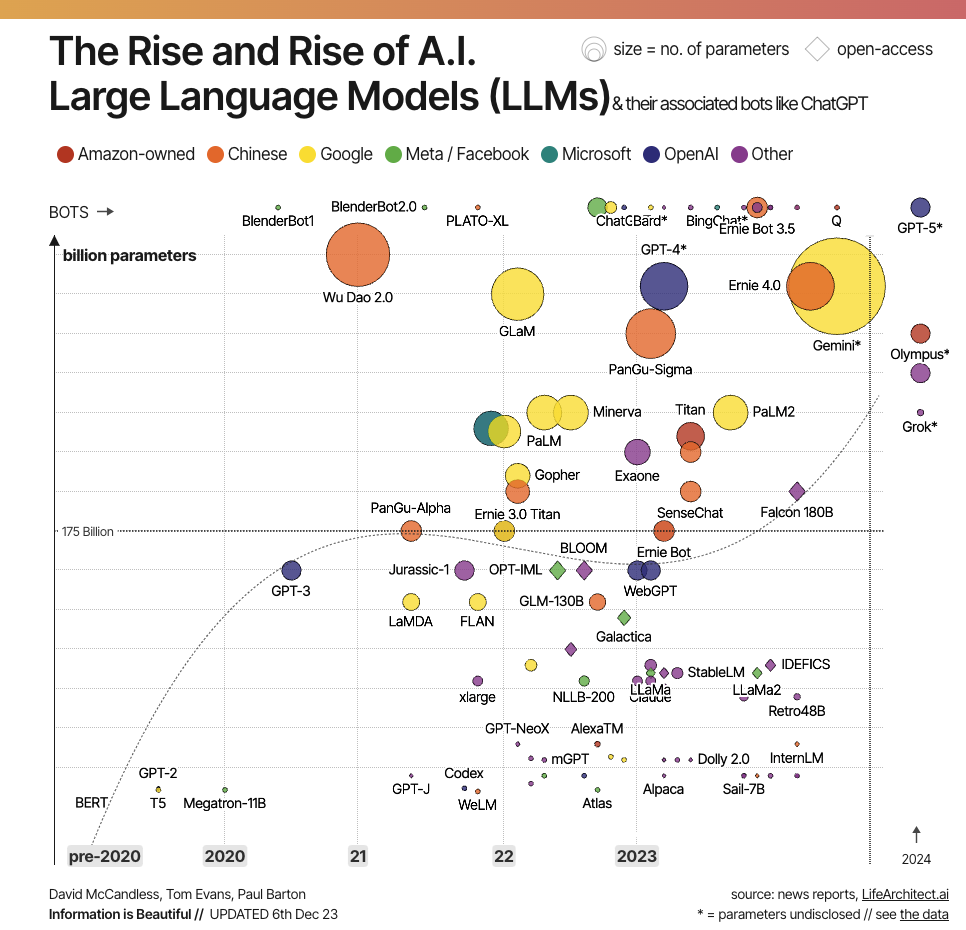
\includegraphics[width=0.6\linewidth,keepaspectratio]{llm120}
\end{center}		

{\tiny (Ref: https://informationisbeautiful.net/visualizations/the-rise-of-generative-ai-large-language-models-llms-like-chatgpt/)}

\end{frame}


% %%%%%%%%%%%%%%%%%%%%%%%%%%%%%%%%%%%%%%%%%%%%%%%%%%%%%%%%%%%
% \begin{frame}[fragile]\frametitle{Overview of LLM}


% \begin{itemize}
% \item Large Language Models (LLMs) are deep neural networks (e.g., GPT-3, BERT) based on the Transformer architecture.
% \item LLMs are foundation models trained on large amounts of unsupervised and unstructured data.
% \item The Transformer architecture consists of an encoder and decoder, both mostly identical with a few differences.
% \item LLMs compute a probability distribution over a vocabulary (list of tokens) given an input prompt.
% \item LLMs have limitations like hallucination and issues in chain of thought reasoning, but recent improvements have been made.
% \item LLMs are trained for statistical language modeling, which involves predicting the next token based on context.
% \end{itemize}

				
% {\tiny (Ref: Overview of Large Language Models - Aman AI)}

% \end{frame}

% %%%%%%%%%%%%%%%%%%%%%%%%%%%%%%%%%%%%%%%%%%%%%%%%%%%%%%%%%%%
% \begin{frame}[fragile]\frametitle{How Large Language Models Work}
  
  % \begin{itemize}
    % \item \textbf{Learning from Lots of Text:} Models like GPT-3 start by reading a massive amount of text from the internet. It's akin to learning from a giant library of information.
    
    % \item \textbf{Innovative Architecture:} These models use a unique structure called a transformer, which enables them to understand and remember vast amounts of information.
    
    % \item \textbf{Breaking Down Words:} They analyze sentences by breaking words into smaller parts, facilitating more efficient language processing.
    
    % \item \textbf{Understanding Words in Sentences:} Unlike simple programs, these models comprehend individual words and their relationships within a sentence, gaining a holistic understanding.
    
    % \item \textbf{Getting Specialized:} Following general learning, the models can be further trained on specific topics, enhancing proficiency in tasks like answering questions or writing about particular subjects.
    
    % \item \textbf{Doing Tasks:} When provided with a prompt (question or instruction), these models use their acquired knowledge to generate intelligent responses. It's akin to having an assistant that comprehends and generates text.
  % \end{itemize}
  
  % {\tiny (Ref: What are Large Language Models(LLMs)? -Suvojit Hore)}



% \end{frame}

% %%%%%%%%%%%%%%%%%%%%%%%%%%%%%%%%%%%%%%%%%%%%%%%%%%%%%%%%%%%
% \begin{frame}[fragile]\frametitle{How Do LLMs Work?}


% \begin{itemize}
% % \item LLMs predict the next token based on previous tokens in an autoregressive manner for generation.
% \item The prompt is tokenized and converted into embeddings (can be non-contextualized like tf-idf or contextualized like w2v)
% \item Layer-by-layer attention and feed-forward computations are performed.
% % \item Decoder models assign logits to words in the vocabulary or output contextualized embeddings for encoder models.
% \item For decoder models, logits are converted into a probability distribution using Softmax.
% \item The probability distribution determines the next word in the generated text.
% \end{itemize}

				
% {\tiny (Ref: Overview of Large Language Models - Aman AI)}

% \end{frame}

%%%%%%%%%%%%%%%%%%%%%%%%%%%%%%%%%%%%%%%%%%%%%%%%%%%%%%%%%%%
\begin{frame}[fragile]\frametitle{How LLMs work?}

  \begin{itemize}
    \item \textbf{Transformer-Based Architecture:}
      \begin{itemize}
        \item Utilizes the Transformer architecture for processing input sequences.
        \item Self-attention mechanism captures long-range dependencies.
      \end{itemize}

    \item \textbf{Pre-training:} 
      \begin{itemize}
        \item Trained on a massive corpus of text data in an unsupervised manner.
        \item Learns contextualized representations of words and phrases.
      \end{itemize}
	  

    \item \textbf{Generative Capabilities:}
      \begin{itemize}
        \item Can generate coherent and contextually relevant text.
        \item Useful for a wide range of natural language understanding and generation tasks.
      \end{itemize}
	  
    \item \textbf{Fine-tuning (Optional):}
      \begin{itemize}
        \item Model can be fine-tuned on specific downstream tasks.
        \item Adaptation to user or domain-specific requirements.
      \end{itemize}

  \end{itemize}

\end{frame}

%%%%%%%%%%%%%%%%%%%%%%%%%%%%%%%%%%%%%%%%%%%%%%%%%%%%%%%%%%%
\begin{frame}[fragile]\frametitle{Transformer Architecture}

  \begin{itemize}
    \item \textbf{Input Representation:} Embedding layer converts input tokens into high-dimensional vectors.


    \item \textbf{Positional Encoding:} Adds positional information to the input embeddings.


    \item \textbf{Multi-Head Self Attention:}
      \begin{itemize}
        \item Allows each token to focus on different parts of the input sequence.
        \item Multiple attention heads capture diverse patterns.
      \end{itemize}

    \item \textbf{Layer Normalization \& Residual/Skip Connections:}
      \begin{itemize}
        \item Stabilizes training using layer normalization.
        \item Residual connections help in mitigating vanishing/exploding gradient problems.
      \end{itemize}

    \item \textbf{Encoder-Decoder Structure (for Sequence-to-Sequence tasks):} In tasks like translation, multiple encoder layers process the input, and then multiple decoder layers generate the output.

    \item \textbf{Output Layer:} Produces the final output sequence.
  \end{itemize}

\end{frame}

%%%%%%%%%%%%%%%%%%%%%%%%%%%%%%%%%%%%%%%%%%%%%%%%%%%%%%%%%%%
\begin{frame}[fragile]\frametitle{Decoder-Only Transformers (e.g., GPT)}

  \begin{itemize}
    \item \textbf{Architecture:} 
      \begin{itemize}
        \item GPT uses a transformer architecture consisting solely of decoder layers.
        \item Decoders attend to the entire input sequence during training and generation.
      \end{itemize}

    \item \textbf{Positional Embeddings:} Incorporates position information to handle sequence order.

    \item \textbf{Self-Attention Mechanism with Masking:}
      \begin{itemize}
        \item Each position attends to all positions in the preceding context.
        \item During training, masking ensures that positions after the current one are not considered.
        \item Prevents the model from peeking at future tokens during generation.
      \end{itemize}

    \item \textbf{Autoregressive Generation:} 
      \begin{itemize}
        \item Generates output tokens one at a time in an autoregressive manner.
        \item Previous tokens influence the generation of subsequent tokens.
      \end{itemize}

  \end{itemize}

\end{frame}

%%%%%%%%%%%%%%%%%%%%%%%%%%%%%%%%%%%%%%%%%%%%%%%%%%%%%%%%%%%
\begin{frame}[fragile]\frametitle{Large Language Models - Comparison}

\begin{center}
\includegraphics[width=\linewidth,keepaspectratio]{chatgpt31}
\end{center}				
{\tiny (Ref: Deus.ai https://www.deus.ai/post/gpt-3-what-is-all-the-excitement-about)}

\end{frame}

%%%%%%%%%%%%%%%%%%%%%%%%%%%%%%%%%%%%%%%%%%%%%%%%%%%%%%%%%%%
\begin{frame}[fragile]\frametitle{LLM Training}
  \begin{itemize}
    \item Training LLMs involves instructing the model to comprehend and generate human-like text.
    \item \textbf{Input Text:} LLMs are exposed to extensive text data from diverse sources like books, articles, and websites.
    \item During training, the model predicts the next word/token based on context, learning patterns and relationships.
    \item \textbf{Optimizing Weights:} The model has weights for parameters reflecting feature significance.
    \item Throughout training, weights are fine-tuned to minimize error, enhancing the model's prediction accuracy.
	\item After initial training, LLMs can be customized for tasks using small sets of supervised data. This process is known as \textbf{fine-tuning}.
    \item \textbf{Fine-tuning Parameters:} LLMs adjust parameter values based on error feedback during predictions. 
    \item The model refines its language understanding by iteratively adjusting parameters, improving token prediction accuracy.
    \item Training may vary for specific LLM types, like those optimized for continuous text or dialogue.
  \end{itemize}
\end{frame}

%%%%%%%%%%%%%%%%%%%%%%%%%%%%%%%%%%%%%%%%%%%%%%%%%%%%%%%%%%%
\begin{frame}[fragile]\frametitle{LLM Performance Factors}
  \begin{itemize}
    \item \textbf{Model Architecture:} LLM performance is influenced by the design and intricacy of its architecture.
    \item \textbf{Dataset Quality:} The quality and diversity of the training dataset shape the model's language understanding.
    \item Training a private LLM demands substantial computational resources and expertise.
    \item Duration ranges from days to weeks, contingent on model complexity and dataset size.
    \item Cloud-based solutions and high-performance GPUs expedite the training process.
    \item LLM training is meticulous and resource-intensive, forming the basis for language comprehension and generation.
  \end{itemize}
\end{frame}

%%%%%%%%%%%%%%%%%%%%%%%%%%%%%%%%%%%%%%%%%%%%%%%%%%%%%%%%%%%
\begin{frame}[fragile]\frametitle{Decoder-Only Transformers (e.g., GPT)}

  \begin{itemize}
    \item \textbf{Architecture:} 
      \begin{itemize}
        \item GPT uses a transformer architecture consisting solely of decoder layers.
        \item Decoders attend to the entire input sequence during training and generation.
      \end{itemize}

    \item \textbf{Positional Embeddings:} Incorporates position information to handle sequence order.

    \item \textbf{Self-Attention Mechanism with Masking:}
      \begin{itemize}
        \item Each position attends to all positions in the preceding context.
        \item During training, masking ensures that positions after the current one are not considered.
        \item Prevents the model from peeking at future tokens during generation.
      \end{itemize}

    \item \textbf{Autoregressive Generation:} 
      \begin{itemize}
        \item Generates output tokens one at a time in an autoregressive manner.
        \item Previous tokens influence the generation of subsequent tokens.
      \end{itemize}

  \end{itemize}

\end{frame}


%%%%%%%%%%%%%%%%%%%%%%%%%%%%%%%%%%%%%%%%%%%%%%%%%%%%%%%%%%%
\begin{frame}[fragile]\frametitle{LLM Real World Use Cases}

\begin{center}
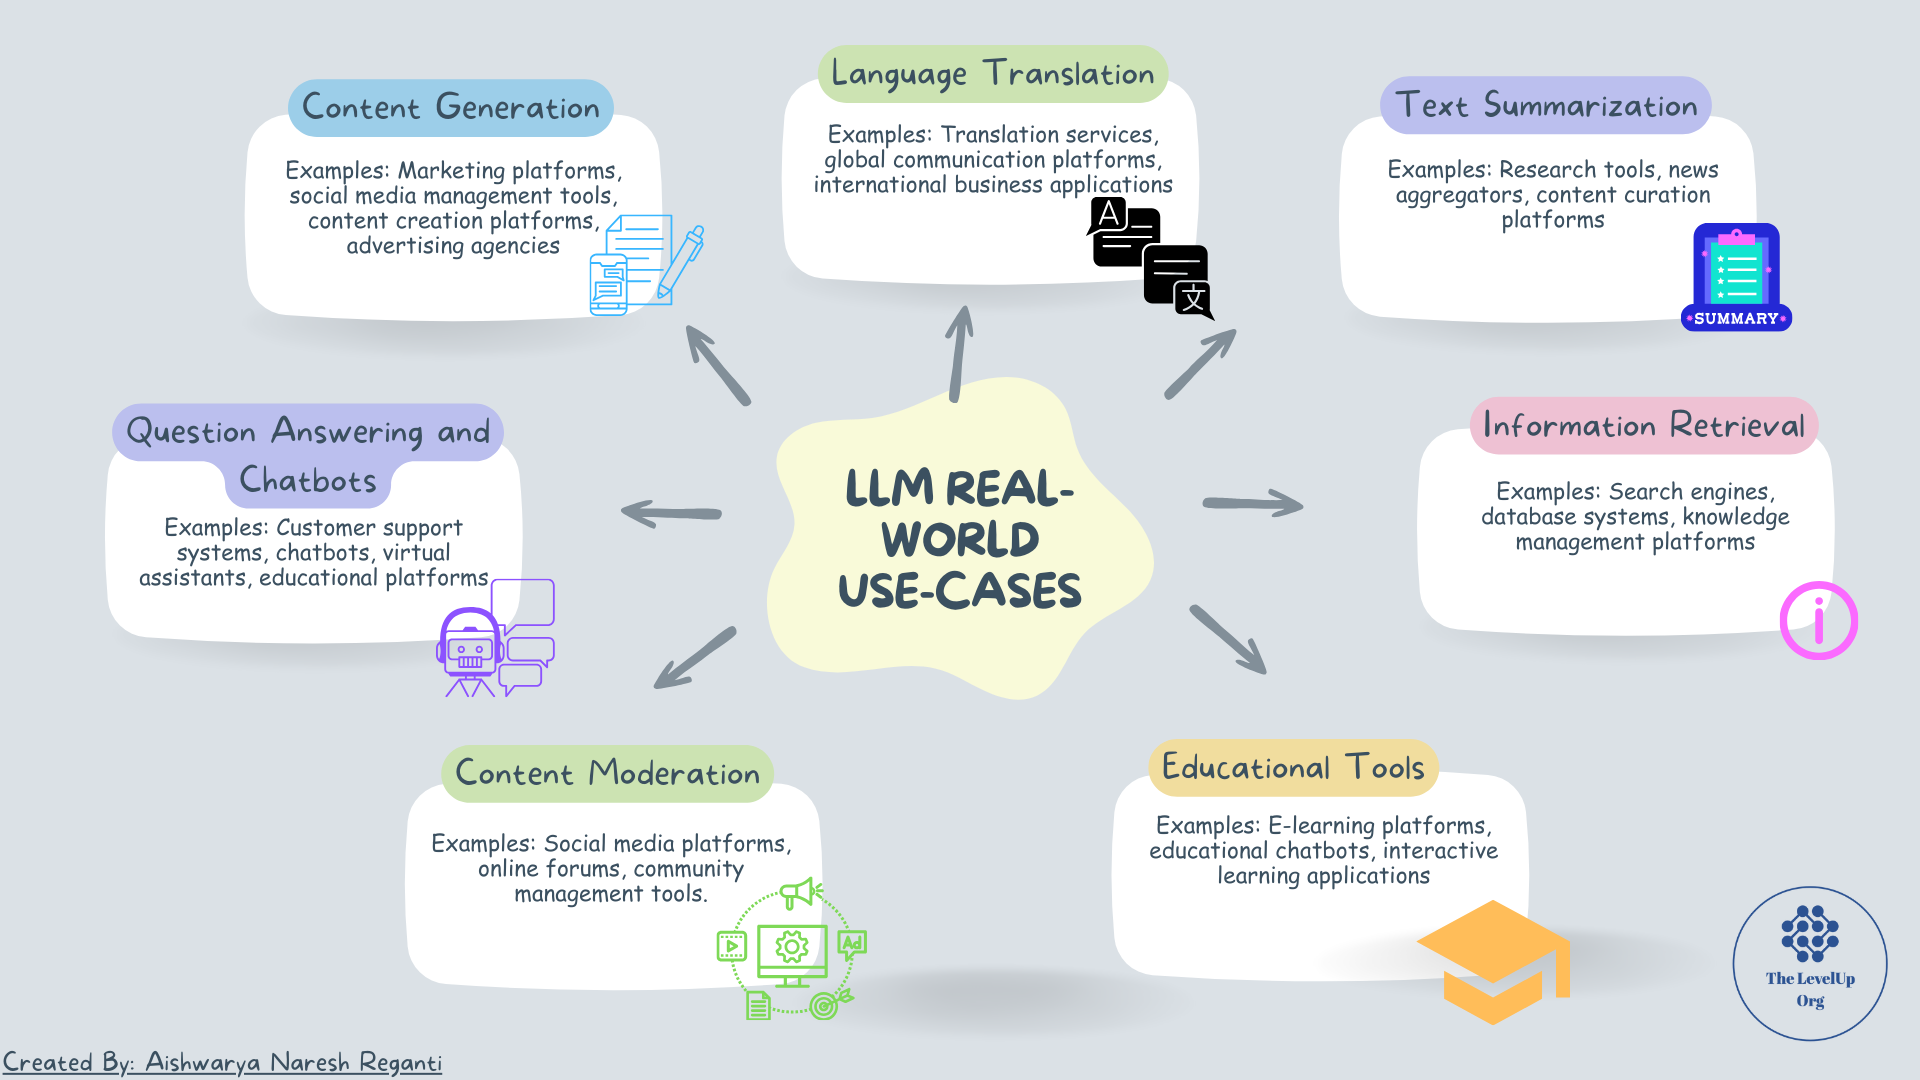
\includegraphics[width=\linewidth,keepaspectratio]{llm121}
\end{center}				

{\tiny (Ref: Applied LLMs Mastery 2024 - Aishwarya Reganti)}

\end{frame}

%%%%%%%%%%%%%%%%%%%%%%%%%%%%%%%%%%%%%%%%%%%%%%%%%%%%%%%%%%%
\begin{frame}[fragile]\frametitle{LLM Real World Use Cases}

\begin{center}
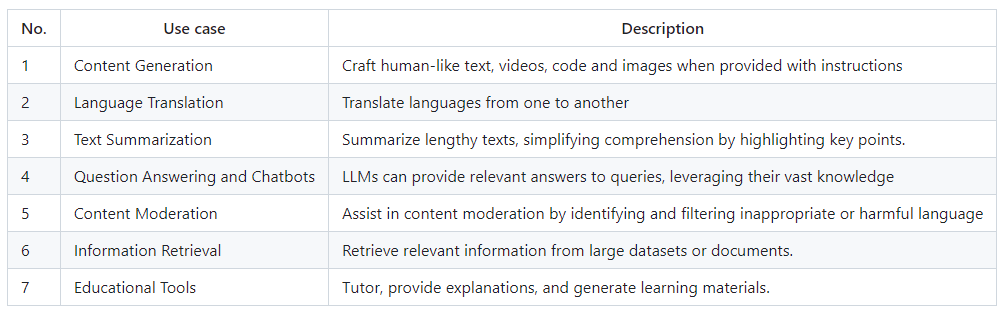
\includegraphics[width=\linewidth,keepaspectratio]{llm122}
\end{center}				

{\tiny (Ref: Applied LLMs Mastery 2024 - Aishwarya Reganti)}

\end{frame}

%%%%%%%%%%%%%%%%%%%%%%%%%%%%%%%%%%%%%%%%%%%%%%%%%%%%%%%%%%%
\begin{frame}[fragile]\frametitle{LLM Challenges}

\begin{center}
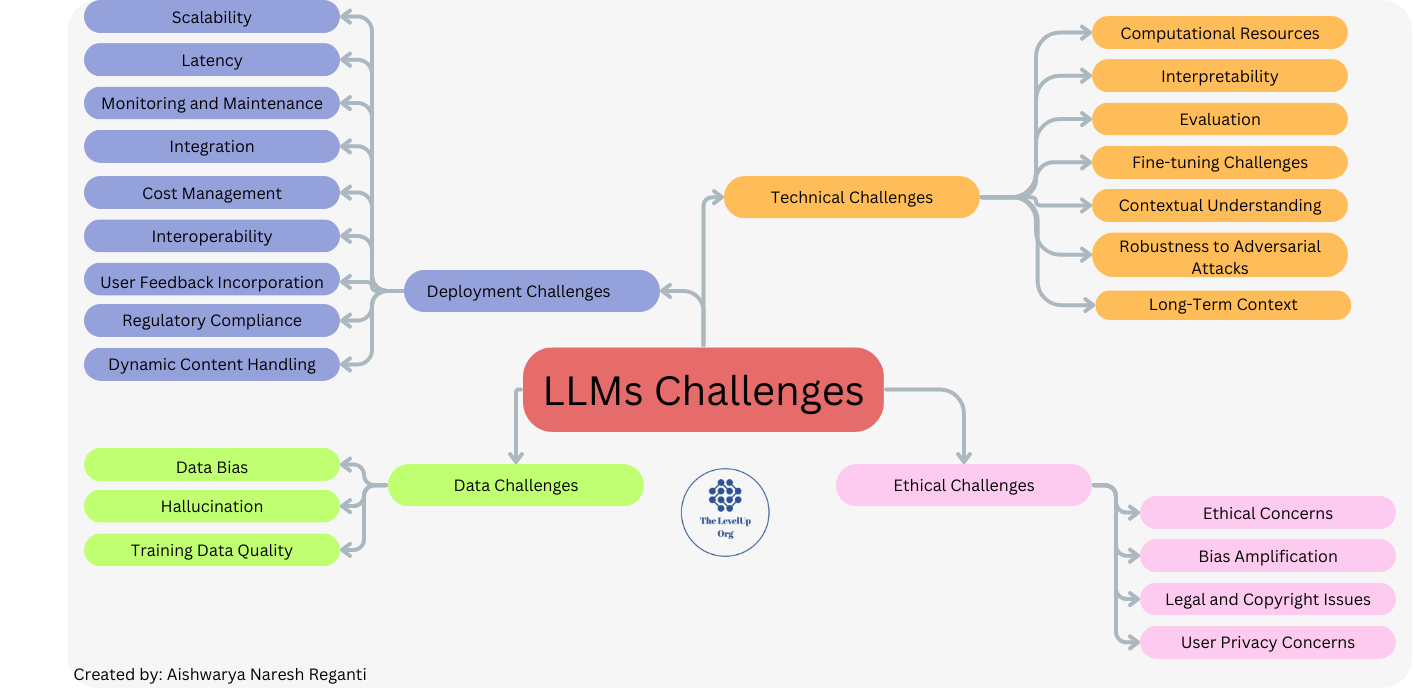
\includegraphics[width=\linewidth,keepaspectratio]{llm123}
\end{center}				

{\tiny (Ref: Applied LLMs Mastery 2024 - Aishwarya Reganti)}

\end{frame}

% %%%%%%%%%%%%%%%%%%%%%%%%%%%%%%%%%%%%%%%%%%%%%%%%%%%%%%%%%%%
% \begin{frame}[fragile]\frametitle{LLM Training Steps}

% At a top-level, here are steps involved in training LLMs:

% \begin{itemize}
% \item Corpus Preparation: Gather a large corpus of text data from various sources.
% Tokenization: Split the text into individual words or subword units (tokens).
% Embedding Generation: Generate embeddings using random initialization or pre-trained embeddings like Word2Vec, GloVe, or FastText.
% Neural Network Training: Train a neural network model on the input tokens.
% \begin{itemize}
% \item For encoder models (e.g., BERT), predict the context of a given word through masked language modeling and next sentence prediction tasks.
% \item For decoder models (e.g., GPT-N), predict the next token in the sequence based on prior context.
% \end{itemize}
% \end{itemize}

				
% {\tiny (Ref: Overview of Large Language Models - Aman AI)}

% \end{frame}

% %%%%%%%%%%%%%%%%%%%%%%%%%%%%%%%%%%%%%%%%%%%%%%%%%%%%%%%%%%%
% \begin{frame}[fragile]\frametitle{Computing Similarity Between Embeddings}


% \begin{itemize}
% \item Encoder models provide contextualized embeddings that enable arithmetic operations for various tasks.
% \item Contextualized embeddings can be used for word similarity by comparing the embeddings of the respective words.
% \item For sentence similarity, the output of the [CLS] token or the average of word embeddings can be used.
% \item Sentence BERT variants of encoder models are preferred for optimal performance on sentence similarity tasks.
% \item Word/sentence similarity measures the semantic equivalence between two words/sentences.
% \item Two common measures of word/sentence similarity exist, which are not considered "distance metrics."
% \end{itemize}

				
% {\tiny (Ref: Overview of Large Language Models - Aman AI)}

% \end{frame}


% %%%%%%%%%%%%%%%%%%%%%%%%%%%%%%%%%%%%%%%%%%%%%%%%%%%%%%%%%%%
% \begin{frame}[fragile]\frametitle{Reasoning}


% \begin{itemize}
% \item Reasoning in LLMs refers to the ability to make inferences using evidence and logic.
% \item There are different types of reasoning, including commonsense reasoning and mathematical reasoning.
% \item Various methods, such as prompting, can be used to elicit reasoning from LLMs.
% \item Determining the extent of reasoning used by LLMs for final predictions is challenging, as separating reasoning from factual information is not straightforward.
% \end{itemize}

				
% {\tiny (Ref: Overview of Large Language Models - Aman AI)}

% \end{frame}


% %%%%%%%%%%%%%%%%%%%%%%%%%%%%%%%%%%%%%%%%%%%%%%%%%%%%%%%%%%%
% \begin{frame}[fragile]\frametitle{GPTs Training}

% GPT: Generative Pre-trained Transformers

% \begin{itemize}
% % \item GPT-1 is trained in a self-supervised manner (learn to predict the next word in text data) and fine-tuned in a supervised learning manner. 
% % \item GPT-2 is trained in a fully self supervised way, focusing on zero-shot transfer
% % \item  GPT-3 is pre-trained in a self supervised manner exploring a bit more the few-shots fine-tuning.
% \item GPT-1 is pre-trained on the BooksCorpus dataset, containing ~7000 books amounting to ~5GB of data
% \item GPT-2 is pre-trained using the WebText dataset which is a more diverse set of internet data containing ~8M documents for about ~40 GB of data
% \item GPT-3 uses an expanded version of the WebText dataset, two internet-based books corpora that are not disclosed and the English-language Wikipedia which constituted ~600 GB of data
% \end{itemize}	 

% \end{frame}

% %%%%%%%%%%%%%%%%%%%%%%%%%%%%%%%%%%%%%%%%%%%%%%%%%%%%%%%%%%%
% \begin{frame}[fragile]\frametitle{GPTs Training compared to human reading}

% \begin{itemize}
% % \item GPT-1 is trained in a self-supervised manner (learn to predict the next word in text data) and fine-tuned in a supervised learning manner. 
% % \item GPT-2 is trained in a fully self supervised way, focusing on zero-shot transfer
% % \item  GPT-3 is pre-trained in a self supervised manner exploring a bit more the few-shots fine-tuning.
% \item GPT-3 was trained on 499B tokens; GPT-4, on 1.4T tokens.
% \item In comparison, if you spent 12 hours a day reading for an entire lifetime (80 years) at average speed (250 words / minute), we would absorb 5.26B words (tokens).
% \item That's a ratio of 100:1 between the training data used for GPT-3 and the amount of data that can ever be read by a human, and 260:1 for GPT-4.
% \end{itemize}	 

% \tiny{(Ref: LinkedIn post by Dr Jennifer Prendki)}

% \end{frame}


% %%%%%%%%%%%%%%%%%%%%%%%%%%%%%%%%%%%%%%%%%%%%%%%%%%%%%%%%%%%%%%%%%%%%%%%%%%%%%%%%%%
% \begin{frame}[fragile]\frametitle{Other Use Cases}
	

% \begin{itemize}
% \item Image: the AI will generate a new image based on your prompt and the image provided.
% \item Embeddings: turn input into a vector representation. It’s very useful when we need to compare the similarity between two texts.
% \item Audio: turn audio into text.
% \end{itemize}	 

% {\tiny (Ref: Techy Stuff 1: Notes on Transformers, LLMs, and OpenAI - Bill)}
			
% \end{frame}


% %%%%%%%%%%%%%%%%%%%%%%%%%%%%%%%%%%%%%%%%%%%%%%%%%%%%%%%%%%%
% \begin{frame}[fragile]\frametitle{Methods to Knowledge-Augment LLMs}

% Let’s look at a few methodologies to knowledge-augment LLMs

% \begin{itemize}
% \item Few-shot prompting: Powerful method for teaching LM desired outputs without weight updates; LM's reasoning and acting abilities tied to provided prompts.
% \item Fine-tuning: Complementary to few-shot prompting; update weights of parameters via supervised learning.
% \item Prompt pre-training: Mixing pre-training data with labeled demonstrations of reasoning to avoid overfitting during fine-tuning; empirical studies on gains compared to separate fine-tuning stage needed.
% \item Bootstrapping: Prompting LM in few-shot setup, discarding examples where actions or reasoning steps didn't lead to correct final prediction.
% \item Reinforcement Learning: Effective for teaching models to reason and act, utilizing supervised learning from human-created prompts.
% \end{itemize}

% {\tiny (Ref: Overview of Large Language Models - Aman AI)}

% \end{frame}

% %%%%%%%%%%%%%%%%%%%%%%%%%%%%%%%%%%%%%%%%%%%%%%%%%%%%%%%%%%%%%%%%%%%%%%%%%%%%%%%%%%
% \begin{frame}[fragile]\frametitle{}
% \begin{center}
% {\Large Example LLMs with Front-Ends}

% \end{center}
% \end{frame}



%%%%%%%%%%%%%%%%%%%%%%%%%%%%%%%%%%%%%%%%%%%%%%%%%%%%%%%%%%%
\begin{frame}[fragile]\frametitle{ChatGPT | GPT3.5/GPT4}


\begin{columns}
    \begin{column}[T]{0.6\linewidth}
		\begin{center}
		\includegraphics[width=\linewidth,keepaspectratio]{promptengg82}

		{\tiny (Ref: The Complete Prompt Engineering for AI Bootcamp (2023))}
		\end{center}	
    \end{column}
    \begin{column}[T]{0.4\linewidth}
		Created by OpenAI
		Access it with code or without (Playground https://platform.openai.com/playground)
    \end{column}
  \end{columns}
\end{frame}

% %%%%%%%%%%%%%%%%%%%%%%%%%%%%%%%%%%%%%%%%%%%%%%%%%%%%%%%%%%%
% \begin{frame}[fragile]\frametitle{GPT3 Features}


		% \begin{center}
		% \includegraphics[width=\linewidth,keepaspectratio]{promptengg83}

		% {\tiny (Ref: The Complete Prompt Engineering for AI Bootcamp (2023))}
		% \end{center}	

% \end{frame}


% %%%%%%%%%%%%%%%%%%%%%%%%%%%%%%%%%%%%%%%%%%%%%%%%%%%%%%%%%%%
% \begin{frame}[fragile]\frametitle{GPT3 Usecases}


		% \begin{center}
		% \includegraphics[width=\linewidth,keepaspectratio]{promptengg84}

		% {\tiny (Ref: The Complete Prompt Engineering for AI Bootcamp (2023))}
		% \end{center}	

% \end{frame}

% %%%%%%%%%%%%%%%%%%%%%%%%%%%%%%%%%%%%%%%%%%%%%%%%%%%%%%%%%%%
% \begin{frame}[fragile]\frametitle{GPT3 Limitations}




% \begin{itemize}
% \item  Unlike ChatGPT, GPT-3 doesn’t store chat history, which can lead to you needing to re-inject the extra context into the
% original prompt.
% \item Tokens are currently limited to 4000 tokens per output. This includes both your initial prompt the text generated
% from ChatGPT.

% \end{itemize}	 

% {\tiny (Ref: The Complete Prompt Engineering for AI Bootcamp (2023))}

% \end{frame}


%%%%%%%%%%%%%%%%%%%%%%%%%%%%%%%%%%%%%%%%%%%%%%%%%%%%%%%%%%%
\begin{frame}[fragile]\frametitle{Bard | Palm 2/Gemini}


\begin{columns}
    \begin{column}[T]{0.6\linewidth}
		\begin{center}
		\includegraphics[width=\linewidth,keepaspectratio]{promptengg85}

		{\tiny (Ref: The Complete Prompt Engineering for AI Bootcamp (2023))}
		\end{center}	
    \end{column}
    \begin{column}[T]{0.4\linewidth}
		Created by Google
		Access it via chat https://bard.google.com/ or encounter it in search results
    \end{column}
  \end{columns}
\end{frame}

% %%%%%%%%%%%%%%%%%%%%%%%%%%%%%%%%%%%%%%%%%%%%%%%%%%%%%%%%%%%
% \begin{frame}[fragile]\frametitle{Bard Features}


		% \begin{center}
		% \includegraphics[width=\linewidth,keepaspectratio]{promptengg86}

		% {\tiny (Ref: The Complete Prompt Engineering for AI Bootcamp (2023))}
		% \end{center}	

% \end{frame}

% %%%%%%%%%%%%%%%%%%%%%%%%%%%%%%%%%%%%%%%%%%%%%%%%%%%%%%%%%%%
% \begin{frame}[fragile]\frametitle{Bard Usecases}


		% \begin{center}
		% \includegraphics[width=\linewidth,keepaspectratio]{promptengg87}

		% {\tiny (Ref: The Complete Prompt Engineering for AI Bootcamp (2023))}
		% \end{center}	

% \end{frame}



% %%%%%%%%%%%%%%%%%%%%%%%%%%%%%%%%%%%%%%%%%%%%%%%%%%%%%%%%%%%
% \begin{frame}[fragile]\frametitle{Meta LLaMA}


% \begin{columns}
    % \begin{column}[T]{0.6\linewidth}
		% \begin{center}
		% \includegraphics[width=\linewidth,keepaspectratio]{promptengg88}

		% {\tiny (Ref: The Complete Prompt Engineering for AI Bootcamp (2023))}
		% \end{center}	
    % \end{column}
    % \begin{column}[T]{0.4\linewidth}
		% Created by Meta and open-sourced / leaked
		% Access via hugging face or lmsys https://chat.lmsys.org/
		% Use one of the fine-tuned models (i.e. Vicuna) for better results
    % \end{column}
  % \end{columns}
% \end{frame}


%%%%%%%%%%%%%%%%%%%%%%%%%%%%%%%%%%%%%%%%%%%%%%%%%%%%%%%%%%%
\begin{frame}[fragile]\frametitle{Meta LLaMA}

\begin{itemize}
\item  Open-Source. Need to build a UX and any advanced functionality around it, and may need to fine-tune it.
\item Many use-cases in the enterprise can’t use OpenAI for fear of sensitive data leaking or being used to train the model (though OpenAI claims to keep API data private).
\item If you have 200+ examples fine-tuning beats prompt engineering for a specific defined task.
\end{itemize}	 

{\tiny (Ref: The Complete Prompt Engineering for AI Bootcamp (2023))}

\end{frame}

%%%%%%%%%%%%%%%%%%%%%%%%%%%%%%%%%%%%%%%%%%%%%%%%%%%%%%%%%%%
\begin{frame}[fragile]\frametitle{Anthropic Claude}


\begin{columns}
    \begin{column}[T]{0.6\linewidth}
		\begin{center}
		\includegraphics[width=\linewidth,keepaspectratio]{promptengg90}

		{\tiny (Ref: The Complete Prompt Engineering for AI Bootcamp (2023))}
		\end{center}	
    \end{column}
    \begin{column}[T]{0.4\linewidth}
		Created by Anthropic 
		https://console.anthropic.com/ or API
		Uses Constitutional AI rather than RLHF
		
		Constitutional AI trains to follow a set of high-level principles or rules, such as a constitution, that specify the desired behavior and outcomes of the system.
		RLHF uses human feedback, such as ratings, preferences, or corrections, to optimize a language model or an agent’s policy using reinforcement learning
    \end{column}
  \end{columns}
\end{frame}

% %%%%%%%%%%%%%%%%%%%%%%%%%%%%%%%%%%%%%%%%%%%%%%%%%%%%%%%%%%%
% \begin{frame}[fragile]\frametitle{Anthropic Claude Features}


% \begin{columns}
    % \begin{column}[T]{0.6\linewidth}
		% \begin{center}
		% \includegraphics[width=\linewidth,keepaspectratio]{promptengg91}

		% {\tiny (Ref: The Complete Prompt Engineering for AI Bootcamp (2023))}
		% \end{center}	
    % \end{column}
    % \begin{column}[T]{0.4\linewidth}
		% 100k Token Window! 
		
		% Use Cases

		% \begin{itemize}
		% \item Large Scale Summarization
		% \item Book Marketing
		% \item Writing Styleguides
		% \end{itemize}	 
    % \end{column}
  % \end{columns}
% \end{frame}

%%%%%%%%%%%%%%%%%%%%%%%%%%%%%%%%%%%%%%%%%%%%%%%%%%%%%%%%%%%
\begin{frame}[fragile]\frametitle{Microsoft Bing | GPT 4}


\begin{columns}
    \begin{column}[T]{0.6\linewidth}
		\begin{center}
		\includegraphics[width=0.8\linewidth,keepaspectratio]{promptengg92}

		{\tiny (Ref: The Complete Prompt Engineering for AI Bootcamp (2023))}
		\end{center}	
    \end{column}
    \begin{column}[T]{0.4\linewidth}
		Powered by OpenAI’s GPT-4
		https://www.microsoft.com/en-gb/bing
    \end{column}
  \end{columns}
\end{frame}


% %%%%%%%%%%%%%%%%%%%%%%%%%%%%%%%%%%%%%%%%%%%%%%%%%%%%%%%%%%%
% \begin{frame}[fragile]\frametitle{Microsoft Bing (GPT 4) Features}


		% \begin{center}
		% \includegraphics[width=\linewidth,keepaspectratio]{promptengg93}

		% {\tiny (Ref: The Complete Prompt Engineering for AI Bootcamp (2023))}
		% \end{center}	

% \end{frame}

% %%%%%%%%%%%%%%%%%%%%%%%%%%%%%%%%%%%%%%%%%%%%%%%%%%%%%%%%%%%
% \begin{frame}[fragile]\frametitle{Microsoft Bing (GPT 4) Use Cases}


		% \begin{center}
		% \includegraphics[width=\linewidth,keepaspectratio]{promptengg94}

		% {\tiny (Ref: The Complete Prompt Engineering for AI Bootcamp (2023))}
		% \end{center}	

% \end{frame}



%%%%%%%%%%%%%%%%%%%%%%%%%%%%%%%%%%%%%%%%%%%%%%%%%%%%%%%%%%%
\begin{frame}[fragile]\frametitle{Falcon}


\begin{columns}
    \begin{column}[T]{0.6\linewidth}
		\begin{center}
		\includegraphics[width=\linewidth,keepaspectratio]{promptengg95}

		{\tiny (Ref: The Complete Prompt Engineering for AI Bootcamp (2023))}
		\end{center}	
    \end{column}
    \begin{column}[T]{0.4\linewidth}
		Access it via HuggingFace transformers library, 
		7B and 40B models as well as instruct fine-tuned
		
		Features:
		\begin{itemize}
		\item Free for commercial use
		\item Open source
		\item Possible to fine-tune
		\end{itemize}	 

    \end{column}
  \end{columns}
\end{frame}

% %%%%%%%%%%%%%%%%%%%%%%%%%%%%%%%%%%%%%%%%%%%%%%%%%%%%%%%%%%%
% \begin{frame}[fragile]\frametitle{Falcon Use Cases}


		% \begin{center}
		% \includegraphics[width=\linewidth,keepaspectratio]{promptengg96}

		% {\tiny (Ref: The Complete Prompt Engineering for AI Bootcamp (2023))}
		% \end{center}	

% \end{frame}

%%%%%%%%%%%%%%%%%%%%%%%%%%%%%%%%%%%%%%%%%%%%%%%%%%%%%%%%%%%
\begin{frame}[fragile]\frametitle{Leader board (Jan 2024)}


		\begin{center}
		% \includegraphics[width=\linewidth,keepaspectratio]{promptengg89}

		% {\tiny (Ref: The Complete Prompt Engineering for AI Bootcamp (2023))}
		
		\includegraphics[width=\linewidth,keepaspectratio]{llm119}
		
		{\tiny (Ref: https://toloka.ai/llm-leaderboard/)}
		\end{center}	

\end{frame}

%%%%%%%%%%%%%%%%%%%%%%%%%%%%%%%%%%%%%%%%%%%%%%%%%%%%%%%%%%%%%%%%%%%%%%%%%%%%%%%%%%
\begin{frame}[fragile]\frametitle{}
\begin{center}
{\Large Want to give it a try? - Hugging Face APIs}

  {\tiny (Ref: What are Large Language Models(LLMs)? -Suvojit Hore)}

\end{center}
\end{frame}

%%%%%%%%%%%%%%%%%%%%%%%%%%%%%%%%%%%%%%%%%%%%%%%%%%%%%%%%%%%%%%%%%%%%%%%%%%%%%%%%%%
\begin{frame}[fragile]\frametitle{Sentence Completion}


\begin{lstlisting}
import requests
from pprint import pprint

API_URL = 'https://api-inference.huggingface.co/models/bigscience/bloomz'
headers = {'Authorization': 'Entertheaccesskeyhere'}

def query(payload):
    response = requests.post(API_URL, headers=headers, json=payload)
    return response.json()
  
params = {'max_length': 200, 'top_k': 10, 'temperature': 2.5}
output = query({
    'inputs': 'Sherlock Holmes is a',
    'parameters': params,
})

print(output)

[{'generated_text': 'Sherlock Holmes is a private investigator whose cases '
                    'have inspired several film productions'}]
\end{lstlisting}

\end{frame}


%%%%%%%%%%%%%%%%%%%%%%%%%%%%%%%%%%%%%%%%%%%%%%%%%%%%%%%%%%%%%%%%%%%%%%%%%%%%%%%%%%
\begin{frame}[fragile]\frametitle{Question Answers}


\begin{lstlisting}
API_URL = 'https://api-inference.huggingface.co/models/deepset/roberta-base-squad2'
headers = {'Authorization': 'Entertheaccesskeyhere'}


def query(payload):
    response = requests.post(API_URL, headers=headers, json=payload)
    return response.json()
  
params = {'max_length': 200, 'top_k': 10, 'temperature': 2.5}
output = query({
    'inputs': {
            "question": "What's my profession?",
            "context": "My name is Yogesh and I am an AI Coach"
        },
    'parameters': params
})

pprint(output)

{'answer': 'AI Coach',
 'end': 39,
 'score': 0.7751647233963013,
 'start': 30}
\end{lstlisting}


\end{frame}


%%%%%%%%%%%%%%%%%%%%%%%%%%%%%%%%%%%%%%%%%%%%%%%%%%%%%%%%%%%%%%%%%%%%%%%%%%%%%%%%%%
\begin{frame}[fragile]\frametitle{Summarization}


\begin{lstlisting}
API_URL = "https://api-inference.huggingface.co/models/facebook/bart-large-cnn"
headers = {'Authorization': 'Entertheaccesskeyhere'}

def query(payload):
    response = requests.post(API_URL, headers=headers, json=payload)
    return response.json()
    
params = {'do_sample': False}

full_text = '''AI applications are summarizing articles, writing stories and 
engaging in long conversations and large language models are doing 
the heavy lifting.

:
'''

output = query({
    'inputs': full_text,
    'parameters': params
})
print(output)

[{'summary_text': 'Large language models - most successful '
                  'applications of transformer models. ...'}]
\end{lstlisting}


\end{frame}

%%%%%%%%%%%%%%%%%%%%%%%%%%%%%%%%%%%%%%%%%%%%%%%%%%%%%%%%%%%%%%%%%%%%%%%%%%%%%%%%%%
\begin{frame}[fragile]\frametitle{}
\begin{center}
{\Large Conclusions, Cautions and What's Next?}
\end{center}
\end{frame}


%%%%%%%%%%%%%%%%%%%%%%%%%%%%%%%%%%%%%%%%%%%%%%%%%%%%%%%%%%%%%%%%%%%%%%%%%%%%%%%%%%
\begin{frame}[fragile]\frametitle{So, What are LLMs?}

  Large Language Models (LLMs) have revolutionized natural language processing, ushering in advancements in text generation and understanding. Key attributes include:

  \begin{itemize}
    \item \textbf{Learning from Extensive Data:} LLMs acquire knowledge from vast datasets, resembling a massive library of information.

    \item \textbf{Grasping Context and Entities:} These models understand context and entities, allowing for a deeper comprehension of language.

    \item \textbf{Proficient User Query Responses:} LLMs excel in responding to user queries, showcasing their ability to apply learned knowledge effectively.

  \end{itemize}

  Despite their versatile applications across industries, ethical concerns and potential biases necessitate a critical evaluation to understand their societal impact.

\end{frame}

% %%%%%%%%%%%%%%%%%%%%%%%%%%%%%%%%%%%%%%%%%%%%%%%%%%%%%%%%%%%%%%%%%%%%%%%%%%%%%%%%%%
% \begin{frame}[fragile]\frametitle{Key Takeaways}

  % \begin{itemize}
    % \item LLMs comprehend complex sentences, relationships between entities, and user intent.
    % \item LLM architecture: embedding, feedforward, recurrent, and attention layers.
    % \item Popular LLMs like Palm and GPT-3, along with open-source alternatives.
    % \item Hugging Face APIs aid in generating text using LLMs.
    % % \item LLMs are anticipated to revolutionize job markets, communication, and society, emphasizing the need for careful consideration of their limitations and ethical implications.
  % \end{itemize}
% \end{frame}

% %%%%%%%%%%%%%%%%%%%%%%%%%%%%%%%%%%%%%%%%%%%%%%%%%%%%%%%%%%%%%%%%%%%%%%%%%%%%%%%%%%
% \begin{frame}[fragile]\frametitle{Large Language Models Training}
  % \begin{itemize}
    % \item Trained on internet data, including dark content.
    % \item Exposure to racist, sexist, and offensive language.
    % \item May regurgitate such language in generated text.
  % \end{itemize}
% \end{frame}

%%%%%%%%%%%%%%%%%%%%%%%%%%%%%%%%%%%%%%%%%%%%%%%%%%%%%%%%%%%%%%%%%%%%%%%%%%%%%%%%%%
\begin{frame}[fragile]\frametitle{Core Beliefs of Large Language Models}
  \begin{itemize}
    \item No inherent "core beliefs."
    \item Word guessers predicting internet-like sentences.
    \item Can write both for and against a topic without belief.
    \item Emulates the most common response in training data.
  \end{itemize}
\end{frame}

%%%%%%%%%%%%%%%%%%%%%%%%%%%%%%%%%%%%%%%%%%%%%%%%%%%%%%%%%%%%%%%%%%%%%%%%%%%%%%%%%%
\begin{frame}[fragile]\frametitle{Truth and Morality in Large Language Models}
  \begin{itemize}
    \item Lack sense of truth or morality.
    \item Tendency to generate words we agree are true.
    \item No guarantee of providing the actual truth.
  \end{itemize}
\end{frame}

%%%%%%%%%%%%%%%%%%%%%%%%%%%%%%%%%%%%%%%%%%%%%%%%%%%%%%%%%%%%%%%%%%%%%%%%%%%%%%%%%%
\begin{frame}[fragile]\frametitle{Mistakes in Large Language Models}
  \begin{itemize}
    \item Prone to mistakes due to inconsistent training data.
    \item Self-attention may not capture all relevant information.
    \item Hallucination: generating words not derived from input.
    \item Preference for common words, small numbers, and specific names.
  \end{itemize}
\end{frame}

%%%%%%%%%%%%%%%%%%%%%%%%%%%%%%%%%%%%%%%%%%%%%%%%%%%%%%%%%%%%%%%%%%%%%%%%%%%%%%%%%%
\begin{frame}[fragile]\frametitle{Auto-regressive Nature of LLMs}
  \begin{itemize}
    \item Auto-regressive models: guesses affect subsequent inputs.
    \item Errors accumulate, potentially compounding mistakes.
    \item No mechanism to "change minds" or self-correct.
    \item Lack the ability to retry or undo prior choices.
  \end{itemize}
\end{frame}

%%%%%%%%%%%%%%%%%%%%%%%%%%%%%%%%%%%%%%%%%%%%%%%%%%%%%%%%%%%%%%%%%%%%%%%%%%%%%%%%%%
\begin{frame}[fragile]\frametitle{Verification of Outputs}
\begin{itemize}
    \item Always verify outputs of large language models.
    \item Assess competence to verify results in high-stakes tasks.
    \item Mistakes in critical tasks may lead to costly decisions.
\end{itemize}
\end{frame}

% %%%%%%%%%%%%%%%%%%%%%%%%%%%%%%%%%%%%%%%%%%%%%%%%%%%%%%%%%%%%%%%%%%%%%%%%%%%%%%%%%%
% \begin{frame}[fragile]\frametitle{Self-Attention and Input Quality}
% \begin{itemize}
    % \item Self-attention enhances specialization in responses.
    % \item Response quality is proportional to input prompt quality.
    % \item Experiment with different prompts to achieve better results.
% \end{itemize}
% \end{frame}

% %%%%%%%%%%%%%%%%%%%%%%%%%%%%%%%%%%%%%%%%%%%%%%%%%%%%%%%%%%%%%%%%%%%%%%%%%%%%%%%%%%
% \begin{frame}[fragile]\frametitle{Conversation with Large Language Models}
% \begin{itemize}
    % \item No real "conversation" as models don't remember past exchanges.
    % \item Input, response, and follow-up treated as fresh inputs.
    % \item Programming trick creates appearance of continuous conversation.
    % \item No guarantee against contradictions in responses.
% \end{itemize}
% \end{frame}

%%%%%%%%%%%%%%%%%%%%%%%%%%%%%%%%%%%%%%%%%%%%%%%%%%%%%%%%%%%%%%%%%%%%%%%%%%%%%%%%%%
\begin{frame}[fragile]\frametitle{Input Size and Memory Limitations}
\begin{itemize}
    \item Large language models have input size limits.
    \item Conversation appears coherent until log size exceeds limit.
    \item Earlier parts of the conversation are deleted, and the model "forgets."
\end{itemize}
\end{frame}

% %%%%%%%%%%%%%%%%%%%%%%%%%%%%%%%%%%%%%%%%%%%%%%%%%%%%%%%%%%%%%%%%%%%%%%%%%%%%%%%%%%
% \begin{frame}[fragile]\frametitle{Problem-Solving and Planning}
% \begin{itemize}
    % \item Large language models don't perform problem-solving or planning.
    % \item Lack specific goals; they have an objective of word prediction.
    % \item No look-ahead mechanism; transformers are backward-looking.
    % \item Large language models can generate plan-like outputs.
    % \item Recognize plans from training data but lack thoughtful consideration.
    % \item No mechanism for considering alternatives or backtracking.
% \end{itemize}
% \end{frame}



%%%%%%%%%%%%%%%%%%%%%%%%%%%%%%%%%%%%%%%%%%%%%%%%%%%%%%%%%%%%%%%%%%%%%%%%%%%%%%%%%%
\begin{frame}[fragile]
  \frametitle{Ethical Considerations}

  \begin{itemize}
    \item Awareness of potential biases in LLMs is crucial for responsible usage.
    \item Continuous evaluation of ethical implications is necessary to mitigate societal risks.
    \item Balancing the benefits of LLMs with ethical concerns ensures responsible deployment.

  \end{itemize}


\end{frame}


%%%%%%%%%%%%%%%%%%%%%%%%%%%%%%%%%%%%%%%%%%%%%%%%%%%%%%%%%%%%%%%%%%%%%%%%%%%%%%%%%%
\begin{frame}[fragile]
  \frametitle{Future Impact}

  \begin{itemize}
    \item LLMs expected to revolutionize domains such as job markets, communication, and society.
    \item Careful use and ongoing development are essential for positive impacts.
    \item Understanding limitations and ethical considerations is vital for responsible integration into various domains.
  \end{itemize}
\end{frame}

%%%%%%%%%%%%%%%%%%%%%%%%%%%%%%%%%%%%%%%%%%%%%%%%%%%%%%%%%%%
\begin{frame}[fragile]\frametitle{Landscape of LLMs \& Quiz}

\begin{itemize}
\item Types of models - Foundation models, LLM, SLM, VLMs, etc.
\item Common LLM terms - Prompts, Temperature, Hallucinations, Tokens, etc.
\item LLM lifecycle stages - Pre-training, Supervised Fine Tuning, RLHF, etc.
\item LLM evaluations - ROUGE, BLEU, BIG-bench, GLUE, etc.
\item LLM architecture - Encoder, Decoder, Transformer, Attention, etc.
\item Retrieval augmented generation - Vector DBs, Chunking, Evaluations, etc.
\item LLM agents - Memory, Planning, ReAct, CoT, ToT, etc.
\item Cost \ efficiency - GPU, PEFT, LoRA, Quantization, etc.
\item LLM security - Prompt Injection, Data poisoning, etc.
\item Deployment \& inference - Pruning, Distillation, Flash Attention, etc.
\item Platforms supporting LLMOps
\end{itemize}	 

{\tiny (Ref: LinkedIn post by Abhinav Kimothi - 23 Jan 2024)}
\end{frame}

% %%%%%%%%%%%%%%%%%%%%%%%%%%%%%%%%%%%%%%%%%%%%%%%%%%%%%%%%%%%
% \begin{frame}[fragile]\frametitle{Types of Models}

% \begin{itemize}
% \item Foundation Models: Designed to be general-purpose, providing a foundation
% for various AI applications. Examples: GPT 3.5, GPT4, Stable Diffusion, Llama, BERT,
% Gemini
% \item Large Language Models (LLMs): Foundation models, trained on the ``Transformer
% Architecture'', that can perform a wide array of Natural
% Language Processing (NLP) tasks like text generation,
% classification, summarization etc. Examples: GPT 3.5, Llama2, Mistral, Falcon
% \item Small Language Models (SLMs): SLMs are like LLMs but with lesser number of trained
% parameters (therefore called ``Small''): Example : TinyLlama, Pythia, Phi-2
% \item Large Multimodal Models (LMMs): not just process and generate text, but also other data modalities
% like image, video, speech, audio, etc. Example : LLaVA, LLaMA-Adapter V2, LAVIN
% \item Vision Language Models (VLMs): Image generation with text input/ Examples : GPT4, Gemini, Mixtral, Flamingo, BLIP, Macaw
% LLM
% \end{itemize}	 

% {\tiny (Ref: LinkedIn post by Abhinav Kimothi - 23 Jan 2024)}
% \end{frame}

